% !TEX root = ../../book.tex

\chapter{Execution Fundamentals}

\section{A Brief History of Stock Trading}
Stoll (2006)~\cite{hstoll} in an instructive essay traces the evolution of trading that started under a tree in 1792 with 24 brokers. This has become later on the New York Stock Exchange (NYSE). Modern electronic technology has changed how trading is done. Now all transactions are carried out though a computer system with little human intervention (see the snapshots of NYSE over two different decades).
	\begin{figure}[!ht]
   	\centering
   	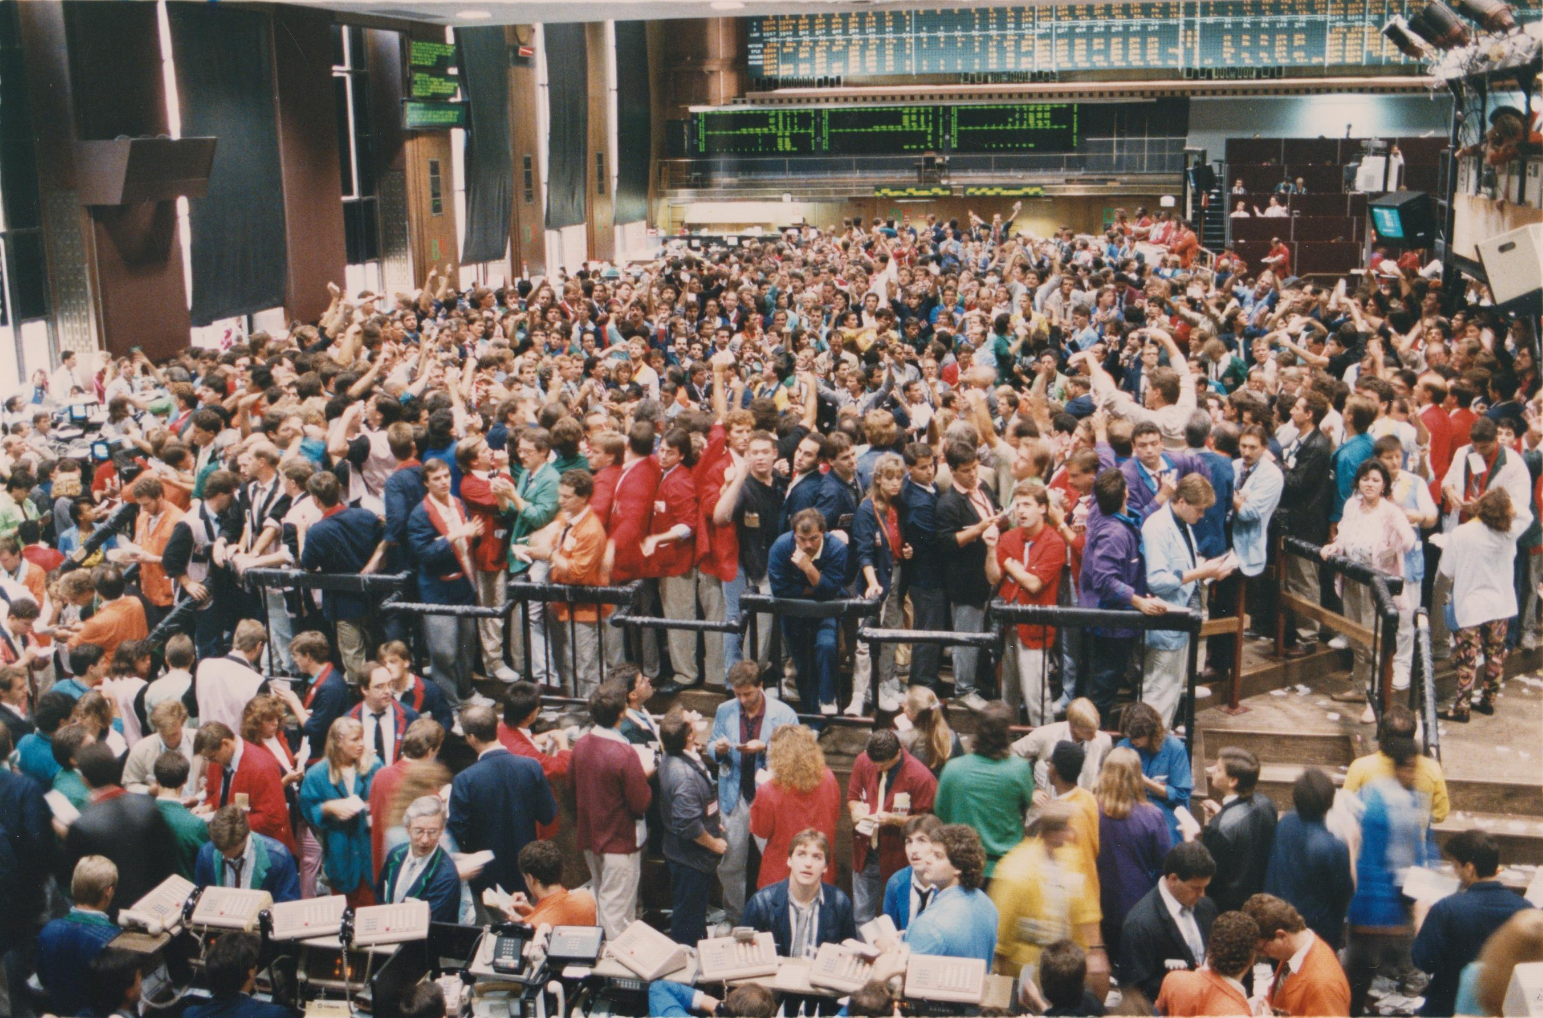
\includegraphics[width=0.9\textwidth]{chapters/chapter_trading_fund/figures/pit_trading.png} 
   	\caption{Treasury bind pit 1989. \label{fig:pittrade}}
	\end{figure}
	\begin{figure}[!ht]
	   \centering
	   \includegraphics[width=0.9\textwidth]{chapters/chapter_trading_fund/figures/electronic_trading.png} 
	   \caption{The NYSE trading floor in August 2008. \label{fig:electrade}}
	\end{figure}
This has also changed how stock market trading is done. The Electronic Communication Networks (ECN) automate the trading process but the fundamental functions of trading are not changed except for the instant dissemination of the demand and supply information to all investors. The identity of traders is kept anonymous. Executions are done fast and very complex orders can now be submitted to the market. The trading costs---both direct such as commissions, brokerage fees, etc. and indirect cost due to price-impact---are expected to be lower. Over the period of two decades (1980--2000), the commissions have have gone down from 1.2\% to 0.2\%. But with higher turnover and thus with increased volume, the total commissions have increased four-fold. The reduction in bid-ask spread although may be primarily due to tick size is accelerated under electronic trading. 


It must be observed that electronic trading does not necessarily imply automated trading. But it has certainly led to more automated trading due to easy execution of the algorithms. Although there is a concern that the traders can game the prices, but computer audit trails can be used to monitor unlawful behaviors. The debate over whether electronification of trading will lead to more consolidation or fragmentation has favored the latter. The apprehension over the possibility of inefficient price formation due to fragmentation is empirically shown not to hold. The order protection rule (SEC 2005) that dictates that an order submitted to any market should get the best of prices in all markets. 

Thus large number of equity and derivative markets are now organized as electronic limit order books. The Electronic Communications Networks (ECNs) in the United States, Hong Kong and Toronto Stock Exchanges are examples of equity markets. Chicago Mercantile Exchange's (CME) Globex platform, Euronext Liffe's centralized limit order book are example of derivative markets. Open limit order books have become popular due to the greater transparency of the market when compared with dealer market settings, that rely upon the information on the dealers' best quotes. The limit order book provides its users to view the depth of the book at various price level away from the best quotes. In dealer market prices for trades beyond the quoted size must be obtained through negotiation with market maker. 


There has been a great deal of interest in studying the information content of an open limit order book and if it helps investors in tracking short-term price predictions. Assuming that the market consists of informed and noise traders, and the informed traders actively submit market orders, Glosten (1994)~\cite{glosten94} and Seppi (1997)~\cite{seppi97} argue that the order book does not contain any information beyond the best bid and best offer. But other studies such as Harris and Panchapagesan (2005)~\cite{harrispan} argue that the order book is informative and specialists better use the book information to their advantage than the traders who routinely place limit orders. In this chapter we discuss the feature of limit order book and various levels of information that have been made available to the investors; the focus is on developing models for studying the dynamics on the book and how the models could be used for high frequency trading. 


An excellent survey paper by Parlour and Seppi (2008)~\cite{parseppi} reviews the issues related to limit order markets. A limit order for any asset `$j$' is an  ex ante pre-commitment $(t,x,p)$ made at time `$t$' to trade `$x$' units at a pre-specified limit price, `$p$'. The order remains valid until it is filled or cancelled. With multiple exchanges, the interactions are quite complex; the dynamic nature of state of the order book and the choice of actions in anticipation of the future states make the limit order placement decisions, $(t,x,p)$ challenging. The key issues in the study of LOB are nicely summarized in Parlour and Seppi (2008)~\cite{parseppi}. They relate to, Price Formulation (How limit order markets differ from dynamic dealer markets?), Liquidity (Implication of the quotes posted at various depths in LOB), Dynamics (Dependencies of Various Trading Decisions), Information Aggregation (How forward-looking is the activity in LOB about future order flow in aggregate?) and Inter-Market Competition (How effective are limit order markets to induce competition and how they handle non-market frictions?). How multiple exchanges can sustain competitive pressure to attract postings to their venues? How do limit order markets help reduce market frictions? These issues are addressed in this chapter but our focus is always on how the information flow through LOB dynamics helps trading decisions. The tools we review here in this chapter can be useful to that end. 


\section{Market Structure and Trading Venues: A Review}
\section{The Mechanics of Trading: The Limit Order Book}

In automated continuous double auction trading system that have become prevalent in financial markets, buyers and sellers submit limit orders electronically; orders are then matched and executed as per time and price priorities.\footnote{Not all exchanges are matching orders following a Price/Time priority algorithm; a key characteristic of the Futures market, for instance, is the existence of pro-rata markets for some fixed income contracts where passive child orders receive fill from aggressive orders based on their size as a fraction of the total passive posted quantity} The unmatched orders are stored in the limit order book (LOB) awaiting further execution. Market orders are orders seeking the best available price and they are executed immediately. Thus, one way or another all executed orders can be considered as marketable orders.


In practice the state of the order book changes quite rapidly due to he multi-agent nature of financial markets and the prevalence of high frequency trading. One can consider there are six types of events, three on either side, that can alter the state of the order book:
	\begin{itemize}
	\item Limit order submission: A limit order is added to the queue at the specified price level.
	\item Limit order cancellation: An outstanding limit order is expired or cancelled and therefore is removed from the LOB.
	\item Marketable order submission: outstanding limit orders at the best price and up to the demanded liquidity price level (in case of pure market order) or up to the limit price (for marketable limit order) are executed against the incoming order and thus removed from the book.
	\end{itemize}


Orders on the buy side are called ``bids'' while those on the sell side are called ``asks.'' The above events are illustrated in Figure~\ref{fig:limbk1} to Figure~\ref{fig:limbk3}. \\
	\begin{figure}[!ht]
	   \centering
	   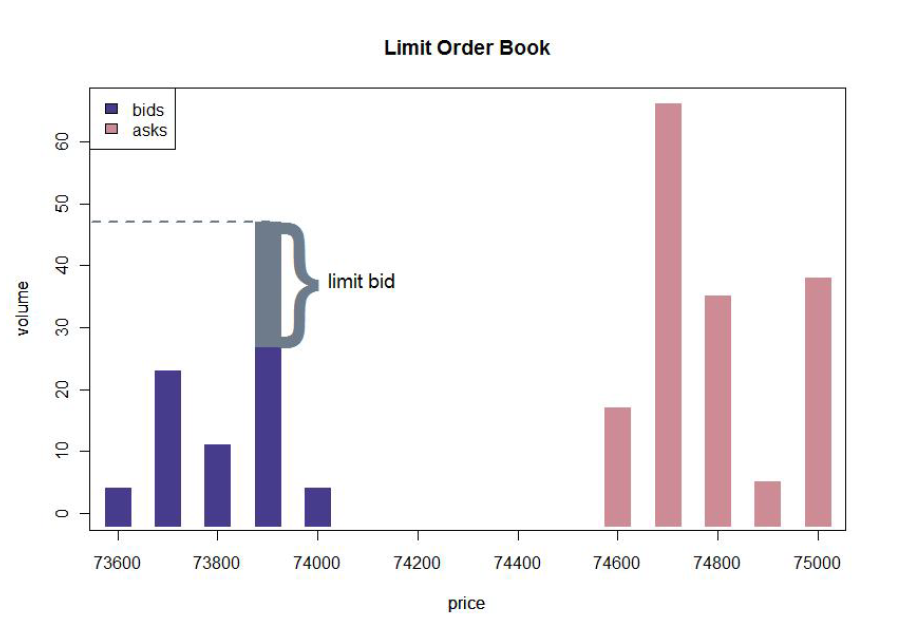
\includegraphics[width=0.9\textwidth]{chapters/chapter_trading_fund/figures/limitbk1.png} 
	   \caption{Limit Order Book---Limit Bid. \label{fig:limbk1}}
	\end{figure}
	\begin{figure}[!ht]
	   \centering
	   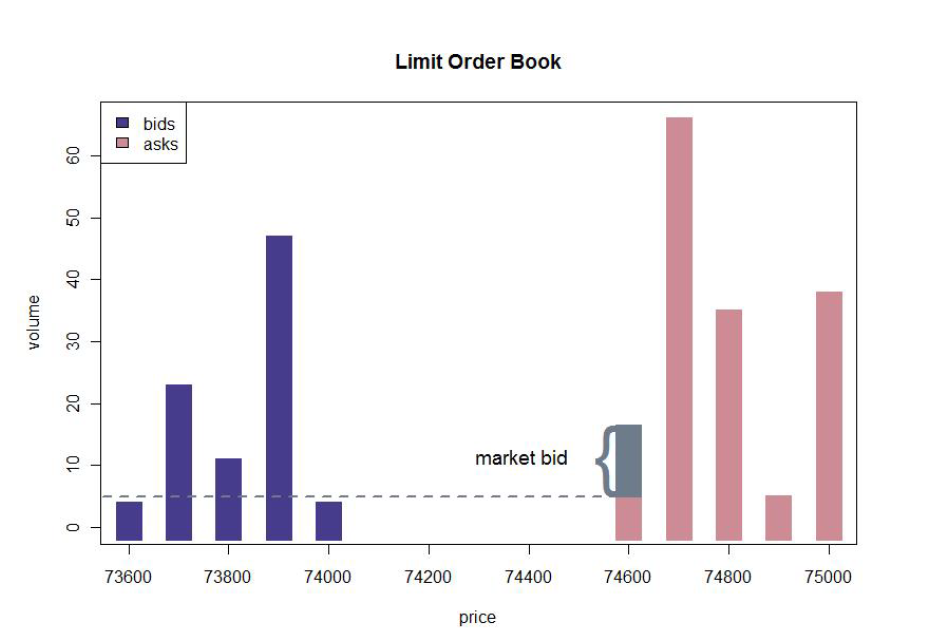
\includegraphics[width=0.9\textwidth]{chapters/chapter_trading_fund/figures/limitbk2.png} 
	   \caption{Limit Order Book---Marketable Bid. \label{fig:limbk2}}
	\end{figure}
When a market (or marketable) order is submitted, it decreases the number of outstanding orders at the opposite best price. For example, if a market bid order arrives, it will decrease the number of outstanding asks at the best price.
	\begin{figure}[!ht]
	   \centering
	   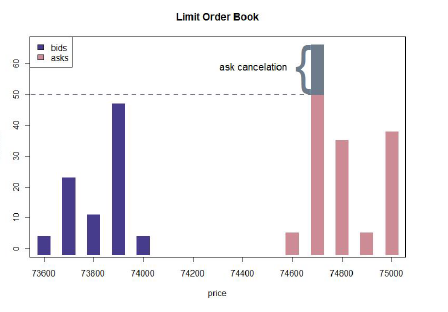
\includegraphics[width=0.9\textwidth]{chapters/chapter_trading_fund/figures/limitbk3.png} 
	   \caption{Limit Order Book---Ask Cancellation. \label{fig:limbk3}}
	\end{figure}
All unexecuted limit orders can be cancelled. When a cancellation occurs, it will decrease the number of outstanding orders at the specified price level. \\


Limit orders make up a significant percentage (70\%) of stock market trading activity. The main advantage of a limit order is that there is no price risk associated to it, that is when the order is executed the limit price is the maximum (for a buy order) or minimum (for a sell order) price that will be achieved. But if the limit order is not marketable, the execution is not guaranteed and the time to get an order executed depends on various market factors. 
The trade off between limit orders and marketable orders depends on the investors need for immediate liquidity and the fill probability of limit orders. The limit price chosen (how deep in the order book is the order placed) as well as the amount of liquidity ahead of the submitted order (how many shares will need to trade before the order gets executed following, for instance, a price/time priority order matching of the exchange) affect both the order fill probability as well as its expected time to fill. These two metrics are of particular relevance for execution algorithms and will be studied in more depth later. 
The execution of limit orders does affect how the quotes are posted and are updated.  
If the size of a market order exceeds the number of shares available at the top of book, it is usually split and is executed at consecutive order book levels until the order is filled. Market orders are usually restricted to be filled within a day and order placed after the markets close might be entered the next day. 
While we mostly considered limit and market orders, it is worth mentioning there exist a wide variety of orders types offered by different exchanges to facilitates certain types of trading activities. Two additional common order types are stop-limit orders and trailing stop orders. The former type is typically used to trade a security at a specified limit price once it traded through a given stop price. If the stock declines in value and trades below or at the stop price, the order will become a limit order rather than a market order. Trailing stop orders follow a similar objective but the stop price trails the best bid or ask by a certain percentage. These order types are primarily used by traders as a protection against sudden adverse market moves. \\

In addition to conditions on price, it is possible to add conditions on the life duration of the order known as Time-in-Force (TIF). The most common types of TIF instructions include Day orders which are valid for the full duration of the trading session and Good-Till-Cancel (GTC) orders which will be placed again on the exchange the next day with similar instructions if they were not fully filled. More sophisticated market participants aiming at achieving greater control over their executions tend to also favor Immediate-or-Cancel (IOC) and Fill-or-Kill (FOK) Time-in-Force instructions. An IOC order will get immediately cancelled back to the sender after reaching the matching engine if it doesn't get immediately a fill, and , in case of a partial fill, the unfilled portion of will also be cancelled, thus preventing it from creating a new price level in the order book. In a Fill-or-Kill scenario, the order gets either filled in its entirety or doesn't get filled at all. This instruction is particularly popular with high frequency market makers and arbitrageurs for which partial fills might result in unwanted legging risk as discussed in the Pairs Trading chapter. \\

Finally, it worth mentioning that some exchanges as well as alternative venues offer the ability of specifying minimum fill sizes whereby a limit order which might be eligible for a fill due to an incoming order at the same price level only receives a fill if the incoming order is larger than a pre-specified number of shares or notional value. This type of instruction is used by market participants as a way of minimizing the number of small fills which carry the risk of excessive information dissemination, in particular in dark pools where they can be used to detect the presence of larger limit orders that would otherwise not be visible to market participants.  

\subsection{How Double Auction Markets Work}

The term double auction refers to the nature of the markets where, unlike a common auction with one auctioneer and many potential buyers, there are many buyers and many sellers.



\subsubsection{Order Types}
\subsubsection{The Open Auction}

The Open Auction is only one of the types of call auctions that are commonly held on exchanges. The term "call auction" explains the liquidity aggregation nature of this event. Market participants are 'called' to submit their quotes to the market place, at a consistent time, in order to determine a matching price that will maximize the amount of shares that can be transacted. \\

INSERT ACTUAL MECHANICS \\

It is worth mentioning that the open auction tends to be considered as a major price discovery mechanism given the fact it occurs after a period of market inactivity when market participants were unable to transact. All new information accumulated overnight will be reflected in the first print of the day, matching buying and selling interests.  

As market participants with better information are more likely to be participating in the open auction with more aggressive orders in order to extract liquidity (and, as such, setting the price), the price discovery mechanism is often considered to be quite volatile and more suited for short-term alpha investors. Similarly, the period immediately following the open auction also tends to be much more volatile than the rest of the day. As a result of which, most markets experience wider spreads while market makers try to protect themselves against information asymmetry by quoting wider bid and offers. 
The increased volatility and wider spread might discouraged certain investors from participating in the market at the open auction and in the period immediately following the open. While this appears to be a reasonable idea from a price risk perspective, it is worth mentioning that for a lot of less liquid stocks (in particular small and mid cap stocks), the open auction can be a significant liquidity aggregation point that even surpasses the close auction. In Australia for instance, the bottom 50\% less liquid stocks have more volume transacted in the open auction than in the close auction. Similarly, in Japan, the less liquid names see more volume trade in the open auction, but also in the afternoon open auction that follows the market lunch break.\\

From a pure execution standpoint, though, the usage of the open auction has to be considered carefully. While this represent a liquidity opportunity, the first print of the day can also have a significant anchoring effect on the stock price for the remainder of the day. So, participating in the open should be considered in light of the liquidity demand of the order: orders that are small enough can likely do without participating in the open auction and the continuous period immediately following; while large orders trying to extract significant liquidity from the market might likely benefit from participating in the open auction.


\subsubsection{Continuous Trading}

THE BORING PART .... INSERT ACTUAL MECHANICS \\


\subsubsection{The Closing Auction}

The Closing Auction tends to be the most popular of the call auctions for a variety of interesting reasons. Firstly, it is the last opportunity (exception made of off-hours trading) when market participants can transact in a relatively liquid environment before being exposed to the overnight period (when new information accumulates, but trades cannot easily take place). Secondly, with the increase in passive investment strategies providing investors with replication of a predetermined benchmark, the closing auction has become a particularly relevant price setting event (most passive funds NAV is based on close prices of the underlying assets). 

For such reasons, the closing auction is particularly important to many investors. From an execution standpoint, it is a major liquidity event that need to be considered carefully. \\

INSERT ACTUAL MECHANICS \\

A large number of Quant and CTA funds are building their investment strategies using daily returns, essentially using the close price as a reference price for their investment decisions. Once their backtesting is built on close price data, they aim at obtaining an execution price equal to or better than the close price when implementing their strategies. 

It also represents a liquidity opportunity for active and passive investors to exchange large amounts of shares. As index constituents get updated on a regular basis (additions, deletions, weight increase/decrease) passive investors need to update their holdings to reflect the optimal composition of the benchmark they track and, in order to minimize their tracking error risk, that update needs to happen as close as possible to the actual update of the underlying benchmark. Consequently, most passive indexers tend to rebalance their portfolios on the same day the underlying index constituents are updated, using the close auction as a reference price, and resulting in significant flows at the close auction. Consequently, active investors looking to build a significant position (or unwinding one) can use these index events as a way of transacting a large amount of shares with low market impact at the close by being a liquidity providers to passive indexers.  



\subsection{Market Data}

Historical market data available to researchers and practitioners alike varied in degrees of granularity over time. From daily trade data (closing price and volume), to tick-by-tick trade and quote data (also known as TAQ data), to full message data, the progressive increase in granularity not only reflects the increase in intraday trading complexity but also opens up the way for more advanced strategies. \\

Initially researchers studying the dynamic of LOB had to content with Trades and Quotes (TAQ) data which provide a time-stamped sequence of trades (Market Orders) and updates in the price and depth of bid and ask quotes. No other information beyond the best bid and the best offer are made available. Moreover, the updates contain changes at the two quotes and were aggregated. The aggregation was clearly a limiting factor as one could not discern the kind of events that led to the changing status of the book. The level II data that became available is a time-stamped sequence of trades and quotes for the top 5-levels of the LOB. This data is little deeper than TAQ data, but was still in aggregated form. But recently made available level III data contains time-stamped sequence of all (except for hidden orders) events that occur in the LOB. Every order is identified by a unique order-id and thus it can be tracked to its lifetime. \\



\subsubsection{Reference Data}

While often overlooked, or merely considered as an after thought in the development of a research platform, reliable reference data is the key foundation of a robust quantitative strategy development.

Commonly used reference data falls into different categories:

\begin{itemize}
\item Symbology mapping: ISIN, SEDOLS, RIC, BBG Tickers, ... .

Quantitative strategies often leverage data from a variety of sources. Different providers key their data with different instrument identifiers depending on asset class or regional conventions, or sometime use their own proprietary identifiers (e.g. Reuter Identification Code - RIC, Bloomberg Ticker). 

It is important to note that such mapping needs to be persisted as point-in-time data and allow for historical "as of date" usage. Over the course of time, some instruments undergo ticker changes (for example from ABC to EDF on date T) without necessarily any particular change on the underlying asset. In such case, market data recorded day-by-day in a trade database will change from being keyed on ABC to being keyed on EDF after the ticker change date T. In order to efficiently backtest strategies over a period of time spanning T, or produce aggregated data (30-day average volume, return over the period, ...), one needs a robust mapping that will allow to seamlessly query the data for the underlying asset such as:

SELECT close price FROM tradeTable WHERE date within [ T-30,  T+10], symbol=EDF


Also: both backward and forward mapping for proper backtesting 

Also, it is not uncommon to have only one of the symbols change on a given day and others remain unchanged for some time, complicating historical data joins even more.

\item Corporate actions: stock dividends and cash dividends (announcement date and ex date), splits, reverse splits, mergers and acquisitions, spin off, rights offer, quote suspension (eg China), free float, shares outstanding.


\item Static data: country, currency, quote factor, sectors (different classifications might be necessary: GICS, ICB, TOPIX 33, ...), trade andquote lot, primary exchange or MIC.

\item Exchange hours, lunch break, holidays, tick tables, DST adjustments to gmt (eg significant impact on intraday liquidity patterns in Brazil), limit up or down constraints and short sell constraints, disrupted days (exchange outage or disruption, market data issues, ...)

\item Primary tickers to composite ticker mapping

\item Market data condition codes to keep/process, dark/lit, blocks, reporting (off book, corrections, auctions, regular, dark, cancelled, Spread, ...)

\item Special day calendars: half days, index rebalance, options and futures expiries, month end, quarter end, Japan SQ, Taiwan trading on Saturdays to make up for golden week, Korea market hour changes for nationwide SAT exam, Gulf countries trading on Sundays instead of Fridays, ... Ramadan in turkey, ... 

\item Futures expiries and handling of most liquid contract, irregular periodicity of contracts (e.g. European index fut monthly expiry vs US ones quarterly, Grains Fut matching the crop cycles), contract size, overnight and day sessions

\item Options chain, expiry calendar

\item Earning calendars (dates and times / backward and forward)

\item Market moving news releases: central banks (FED, ECB, BOE, SNB, BOJ,...), non farm payrolls, crude inventories, PMI, specialized sector events such as FDA results for the healthcare and biotech sectors  .... (Dates and times / backward and forward)

\item ticker changes 

\item Related tickers: dual listed/fungible securities in US and Canada, local and foreign boards in Thailand, 

\item Latency tables (routing, market data collection)

\item composites: time series of constituents, time series of divisor (eg change in free float,...), time series of cash components, mapping to underlying ticker, 

\end{itemize}

\subsubsection{Fundamental Data}

\begin{itemize}
\item key ratios: EPS, P/E, P/B, ...
\item Analyst recommendations, consensus, price targets
\item Earnings consensus
\item Holders // check FINRA/SEC filing forms
\item Insiders Purchase/Sale // check FINRA/SEC filing forms
\end{itemize}

\subsubsection{Daily Statistics}

\begin{itemize}
\item Open, High, Low, Close (OHLC) / Prev Close Price and Date (for computation efficiency such as overnight gap: but needs careful 'adjust=True...), last before close Time/Price
\item Volume + lit/dark breakdown
\item VWAP
\item Short Interest / utilization / days-to-cover
\item Auctions volume (up to 4 of them, + liquidity / intraday ones)
\item Spread (avg, med, twavg) --> or better: parametrized distribution which can then be used in a Bayesian update setup
\item Number of trades
\item Trade size (avg, med) --> or better: parametrized distribution which can then be used in a Bayesian update setup
\item Number and frequency of quote updates 
\item Top of book size
\item Depth of book (price and size)
\item Ticking time (avg, med) --> or better: parametrized distribution which can then be used in a Bayesian update setup
\item Futures and Options:
\begin{itemize}
\item Open Interest
\item Greeks 
\item Implied Vol
\item Basis / dividends estimates
\item Fair Value
\end{itemize}

\item Index-level data for relative measures: OHLC, Overnight gap, ..., benchmark rates (repo, 2y, 10y, 30y?)
\item Asset Class Specific: FI, FX, Credit
\begin{itemize}
\item Yield
\item CDS Spread
\item Closed End Fund: premium / discount
\item USDollar Index
\end{itemize}

\end{itemize}

Can also include pre-computed aggregated X-day trailing data (essentially for computation efficiency in backtest), in particular for normalisation purposes (eg size as a percentage of ADV, spread in relation to long-term average, ...)
\begin{itemize}

\item X-day volatility
\item X-day ADV / Avg auction Volume
\item Beta (full, up-days/down-days) wrt index or sector
\item Correlation to reference index
\end{itemize}

--> Aggregated data need to fully support the peculiarities described in the Reference Data section (for instance: existence of special or event days which, if included, can significantly skew intraday distribution of values; mishandling of market asynchronicity resulting in inaccurate sensitivities computations such as beta or correlation)

\subsubsection{Bin Data}

Aggregated bar data....
Particularly useful to detect seasonalities eg Spread size shrinking in the post-open price discovery period and for quick backtesting of intraday trading strategies

\subsubsection{Level 1: Trade, Quotes, BBO and NBBO}

Superbook \\
Trade time, trade exch time, trade source time \\
Price, size, bid ask price size \\
Quote time, exch time, source time \\
Trade status \\
LULD indicator \\
Qualifiers TRADES AND QUOTES \\
Part ID

\subsubsection{Level 2: Market Depth}


\subsubsection{Level 3: Orders}

--> mention that for generalisation purposes we take the example of US Level 3 data, in particular w.r.t. Table 8.1  \\

\noindent\textbf{Description of Level III data:} The dataset consist of activities during the entire trading session, including early and late hours from 6:00~A.M. to 8:00~P.M. EST in a trading day. It provides intraday depth book activity for 12000 tickers from major national exchanges: Nasdaq, Direct Edge, NYSE, ARCA and BATS (exact number of exchanges depends on the historical period). All messages are consolidated into one file ordered by timestamp. This data allows to build a full national depth book at any moment intraday. The description of the level III data is given in Table~\ref{tab:level3data}. \\
	\begin{table}[!ht]
	\centering
	\begin{tabular}{lp{0.8\textwidth}} \hline
	Variable & Description \\
	& \\
	Timestamp: & Number of milliseconds after the midnight. \\
	& \\
	Ticker: & Equity symbol (up to 8 characters) \\
	& \\
	Order: & Unique order ID. \\
	& \\
	T & Message type. Allowed values: \newline \begin{minipage}[t]{0.6\textwidth} \begin{itemize} \item ``B''---Add buy order \item ``S''---Add sell order \item ``E''---Execute outstanding order in part \item ``C''---Cancel outstanding order in part \item ``F''---Execute outstanding order in full \item ``D''---Delete outstanding order in full \item ``X''---Bulk volume for the cross event \item ``T''---Execute non-displayed order \end{itemize} \end{minipage} \\
	& \\
	Shares & Order quantity for the ``B'', ``S'', ``E'', ``X'', ``C'', ``T'' messages. Zero for ``F'' and ``D'' messages. \\
	& \\
	Price & Order price, available for the ``B'', ``S'', ``X'' and ``T'' messages. \newline Zero for cancellations and executions. The last 4 digits are decimal digits. The decimal portion is padded on the right with zeros. The decimal point is implied by position; it does not appear inside the price field. Divide by 10000 to convert into currency value. \\ 
	& \\
	MPID & Market Participant ID associated with the transaction (4 characters) \\
	& \\
	MCID & Market Center Code (originating exchange---1 character) 
	\end{tabular}
	\caption{Level III data \label{tab:level3data}}
	\end{table}
	

\noindent\textbf{Special types of orders:} While the display and issuance of new ID to the modified order varies from exchange to exchange, we provide a brief description of these orders below:

\begin{enumerate}[1.]
\item Order subject to price sliding: the execution price could be one cent worse than the display price at NASDAQ; it is ranked at the locking price as a hidden order, and displayed at the price one minimum price variation (normally 1 cent) inferior to the locking price. New order ID will be used if the order is replaced as a display order. At other exchanges the old order ID will be used.

\item Pegged order: Based on NBBO, not routable, new timestamp upon re-pricing, display rules vary over exchanges.

\item Mid-point peg order: Non-displayed, can result in half-penny execution.

\item Reserve order: displayed size is ranked as a displayed limit order and the reserve size is behind non-displayed orders and pegged orders in priority. The minimum display quantity is 100 and this amount is replenished from the reserve size when it falls below 100 shares. A new timestamp is created and the displayed size will be re-ranked upon replenishing.

\item Discretionary order: displayed at one price while passively trading at a more aggressive discretionary price. The order becomes active when shares are available within the discretionary price range. Ranked last in priority. The execution price could be worse than the display price.

\item Intermarket sweep order: order that can be executed without the need of checking the prevailing NBBO.  
\end{enumerate}


Some key measures of the LOB are: relative position of an order from the top position of the side (buy or sell), the depth which is the total number of shares at a given price and the depth profile of the book reflects the depth of both prices. Large market orders can shift the bid and ask prices. If the limit price of a new order crosses the best price on the opposite side of the book, it is executed immediately and these are termed as crossing or marketable limit orders. These are used at times to explore the existence of hidden orders.


The limit order book data provides a rich source of information to better understand the market microstructure. The information is also useful for developing trading strategies. Some key issues that may be explored are:

\begin{itemize}
\item The pattern of inter-arrival times of various events.
\item Arrival and cancellation rates as a function of distance from nearest touch price.
\item Arrival and cancellation rates as a function of other available information, such as in the queue on either side of the book.
\end{itemize}

The key issues from the trading point of view are:

\begin{itemize}
\item What is the impact of market order on the limit order book?
\item What are the chances for a limit order to move up the queue from a given entry position?
\item What is the probability of making the spread?
\item What is the direction of the price movement in short duration?
\end{itemize}

\section{The Dynamics of Trading: Market Micro-structure}

Market structure constraints imposed on execution:

\begin{itemize}
\item tick sizes
\item Short sell rules
\item Long queue names
\item 10b-18 rule in US equity
\item Pro-rata markets
\end{itemize}

\section{Execution and its components}
\subsection{Benchmarks}

\begin{itemize}
\item Arrival
\item Inline
\item Full day or Period VWAP
\item Close
\item "All of the above" while completing as much as possible
\end{itemize}

Additional metrics considered for execution performance:
\begin{itemize}
\item completion rate
\item Make/take ratio
\item Mean vs Variance of performance...
\end{itemize}

The benchmark represents a quantitatively measurable observation of the execution objective, which needs to be translated into a series of actual trading actions which are described below


\subsection{Scheduling}

The Macro Trader --> ANSWERS THE QUESTION: How much should I trade in each period?

\begin{itemize}
\item Auctions: to partake or not to partake?
\item Spread Cost vs Liquidity Reward in the "price discovery" period post-open
\item Intraday volume patterns (see next chapter). The value of total day forecast vs intraday distribution?
\item Weekly seasonalities: Monday's are price discovery days, Wed are great?
\item Special days: index events and expiries, quoting deeper at times of news release, ...
\end{itemize}


\subsection{Order Placement (Lit and Dark)}

The Micro Trader --> ANSWERS THE QUESTION: At what price should I trade?

Lit and Dark order placements present different challenges. While lit executions are directly observable and can be observed in public market data feeds, dark executions tend to be reported in aggregate, thus making attribution of actual execution venue more challenging. For instance, if solely observed from market data, dark executions in the US cannot be directly attributed one of the non-displayed venues. However, if observed from the point of view of an executing entity (through execution fills received), one can obtain sensored observations of the available -- otherwise invisible -- liquidity (I.e. When receiving a fill for X shares one knows there was at least X shares available to trade on the other side).

\begin{itemize}
\item Lit Order Placement logic:

\item Dark Order Placement logic: the question one needs to answer here is: given X shares to execute and Y available venues, what is the combination of shares sent to different venues that maximizes the fill probability and minimizes the time to fill?

\end{itemize}


\subsection{Order Routing}

The Smart Order Router --> ANSWERS THE QUESTION: Where should I trade in a fragmented marketplace?

This is only a particular concern in markets that present a significant level of fragmentation, such as the US equity market. 

\begin{itemize}
\item Probability of Fill

\item Time to fill
\end{itemize}


\subsection{RFQ Markets}
What happens in other asset classes???